\documentclass{standalone}

\usepackage{hyperref}
\usepackage{tikz}
\usetikzlibrary{
  arrows,
  calc,
  decorations.pathmorphing,
  decorations.pathreplacing,
  decorations.markings,
  fadings,
  positioning,
  shapes,
  arrows.meta
}
\pgfdeclareradialshading{glow}{\pgfpoint{0cm}{0cm}}{
  color(0mm)=(white);
  color(5mm)=(white);
  color(9mm)=(black);
  color(10mm)=(black)
}

\begin{tikzfadingfrompicture}[name=glow fading]
  \shade [shading=glow] (0,0) circle (1);
\end{tikzfadingfrompicture}

\ifpdf
% Ensure reproducible output
\pdfinfoomitdate=1
\pdfsuppressptexinfo=-1
\pdftrailerid{}
\hypersetup{
  pdfcreator={},
  pdfproducer={}
}
\fi

\begin{document}

\begin{tikzpicture}
  \node at (-9.8, 0) {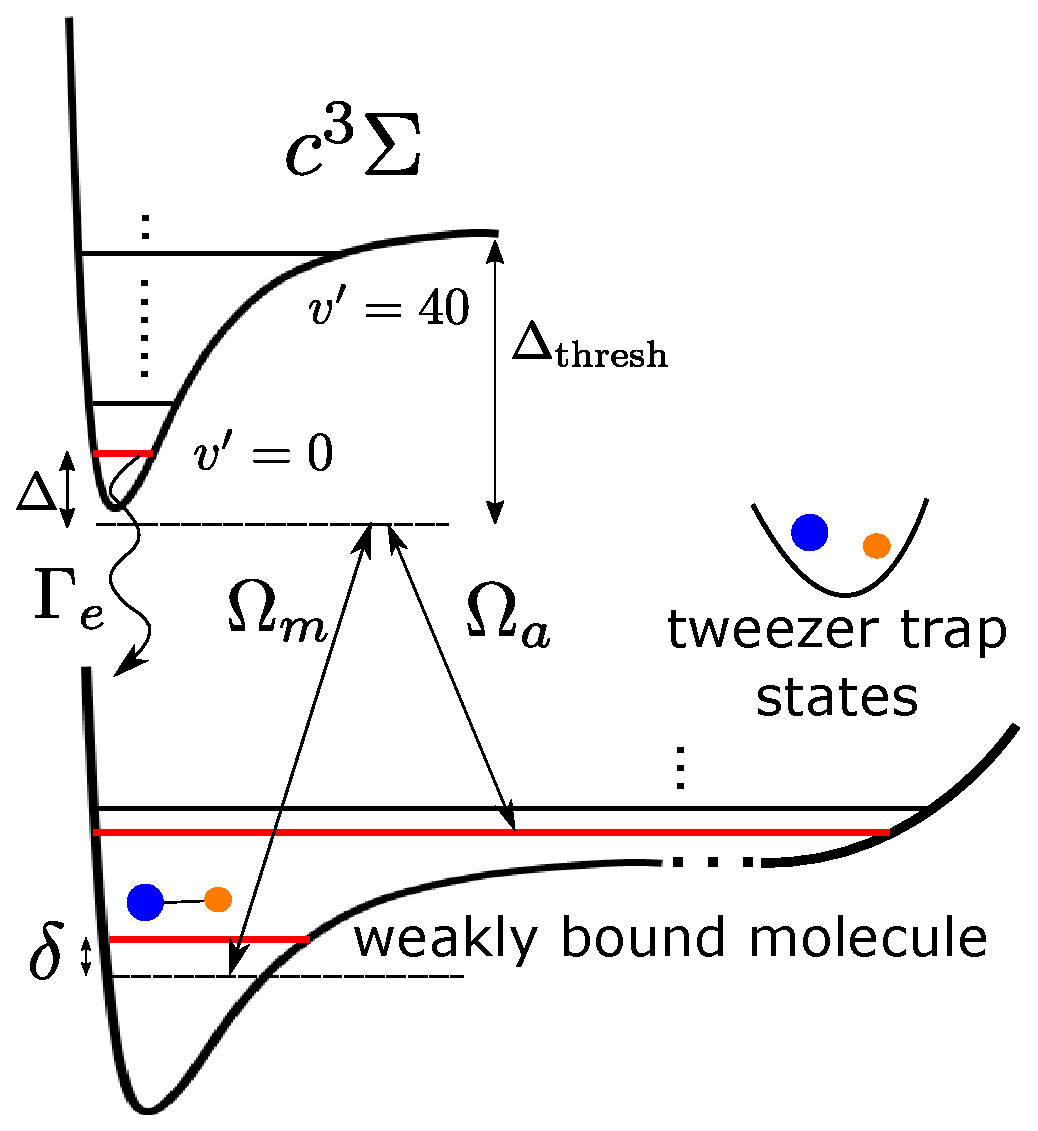
\includegraphics[width=4.5cm]{RamanTransferScheme_v5.eps}};
  \node at (-11.4, 2.2) {\footnotesize (\textbf{a})};
  \node at (-4.35, 0) {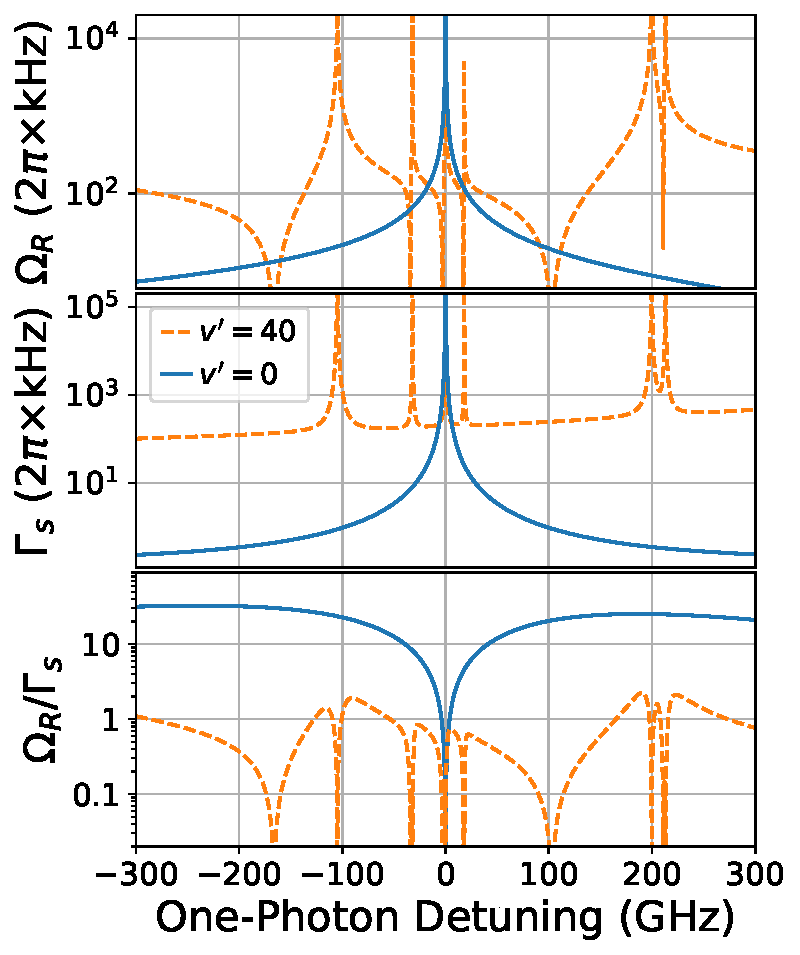
\includegraphics[width=5.7cm]{raman_v0_vhi.pdf}};
  \node at (-5.9, 3.0) {\footnotesize (\textbf{b})};
  \node at (1.4, 0) {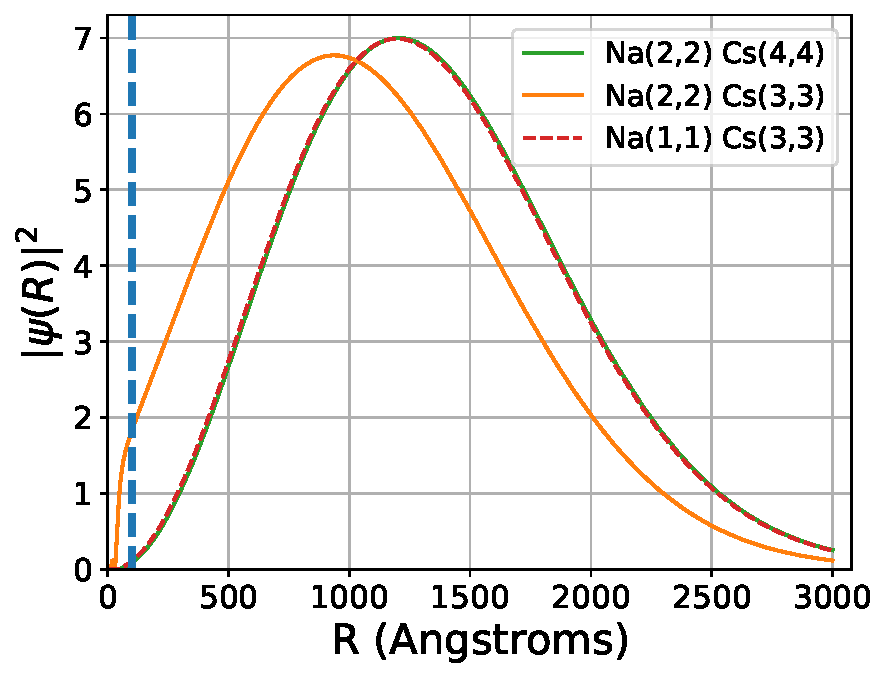
\includegraphics[width=5.7cm]{wavefunction.pdf}};
  \node at (-1.25, 1.9) {\footnotesize (\textbf{c})};
\end{tikzpicture}

\end{document}
